\documentclass[12pt]{article}
\setlength\headheight{14.5pt}
\title{Homework}
\author{Frederick Robinson}
\date{9 February 2010}
\usepackage{amsfonts}
\usepackage{fancyhdr}
\usepackage{amsthm}
\usepackage{graphicx}
\pagestyle{fancyplain}

\begin{document}



\lhead{Frederick Robinson}
\rhead{Math 368: Optimization}

   \maketitle

\setcounter{tocdepth}{2} 

\tableofcontents

\section{Book Problems}

\subsection{Problem 9.2.8}
\subsubsection{Question}
Minimize 
\[ 5 x_1 + 3 x_2\]
subject to 
\[2x_1+5x_2 \geq 10\]
\[3x_1+x_2 \geq 6 \]
\[x_1+7 x_2 \geq 7\]
and 
\[x_1 \geq 0, x_2 \geq 0\]
\subsubsection{Answer}
We begin by observing that, since it contains the point $(100,100)$  the feasible set is nonempty. Moreover we see that the objective function is bounded below by $f(0,0)=0$ since for a smaller value we would need negative $x_1$ or $x_2$, but these are excluded from the feasible set.

We know therefore that the optimum occurs, and moreover that it is at the ``corners" and convex linear combinations of said. So, to compute the optimum we will evaluate the objective function at each of these corners. Towards this we compute each pairwise intersection of functions.
\[
\left(\frac{20}{13},\frac{18}{13}\right)
\left(\frac{35}{9},\frac{4}{9}\right)
(0,2)
(5,0)
\left(\frac{7}{4},\frac{3}{4}\right)
(0,6)
(2,0)
(0,1)
(7,0)
(0,0)
\]

Now we need to check which of these is actually in the feasible set. Doing so reveals that the only ones which are feasilbe are 
\[
\left(\frac{20}{13},\frac{18}{13}\right)
\left(\frac{35}{9},\frac{4}{9}\right)
(0,6)
(7,0)
\]

Evaluating the function at these points we get
\[
f\left(\frac{20}{13},\frac{18}{13}\right)=\frac{154}{13}\approx 11.8462\quad
f\left(\frac{35}{9},\frac{4}{9}\right)=\frac{187}{9}\approx 20.7778
\]
\[
f(0,6)=18\quad
f(7,0)=35
\]
and by inspection we identify that the minimum of the function on the feasible set occurs as
\[f\left(\frac{20}{13},\frac{18}{13}\right)=\frac{154}{13}\]

\subsection{Problem 9.2.12}
\subsubsection{Question}
Mark each statement True of False. Justify each answer.
\begin{enumerate}
\item If a canonical linear programming problem does not have an optimal solution, then either the objective function is not bounded on the feasible set $\mathcal{F}$ or $\mathcal{F}$ is the empty set.
\item If $\overline{x}$ is an optimal solution of a canonical linear programming problem, then $\overline{x}$ is an extreme point of the feasible set.
\end{enumerate}
\subsubsection{Answer}
\begin{enumerate}
\item  True

Theorem 6 state: ``If the feasible set $\mathcal{F}$ is nonempty and if the objective function is bounded above on $\mathcal{F}$, then the canonical linear programming problem has at least one optimal solution. Furthermore, at least one of the optimal solutions is an extreme point of $\mathcal{F}$. "

This is merely the contrapositive of the statement in question. Thus the statement is true.
\item False

This statement is not true. We know in particular that convex combinations of optimal solutions can be optimal, and that more than one extreme point may be optimal. Thus solutions along the ``edge" connecting two optimal extreme solutions are also optimal, yet these points are not themselves extreme points. For a particular counterexample see Part \ref{ce}.
\end{enumerate}


\section{Supplemental Problems}

\subsection{Problem LP.1}
\subsubsection{Question}
Show graphically that the following linear program does not have a unique solution:
\[ \begin{array}{ll} \mathrm{Maximize} & 30 x + 40 y \\
\mathrm{Subject\ to:} & 3x+4y \leq 48\\
& x+y \leq 14\\
& 0 \leq x, 0 \leq y.\\
\end{array}
\]
\subsubsection{Answer}\label{ce}
The following depict the feasible set, and the function evaluated on the feasible set respectively. Intuitively, each value on the ``edge" from $(0,12) $ to $(8,6)$ maximizes the objective function since it is ``highest" on each such value.
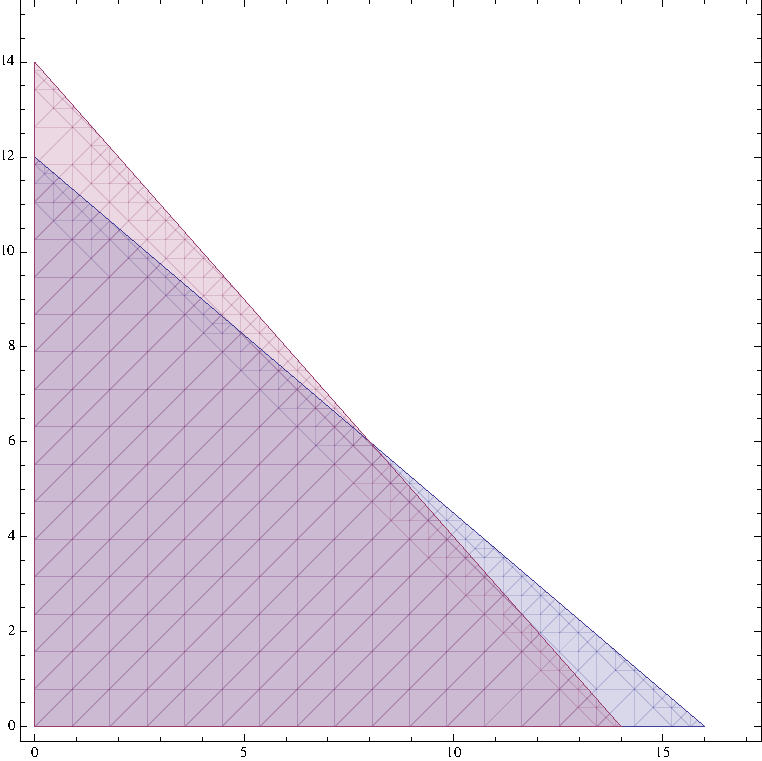
\includegraphics{feasibleset}

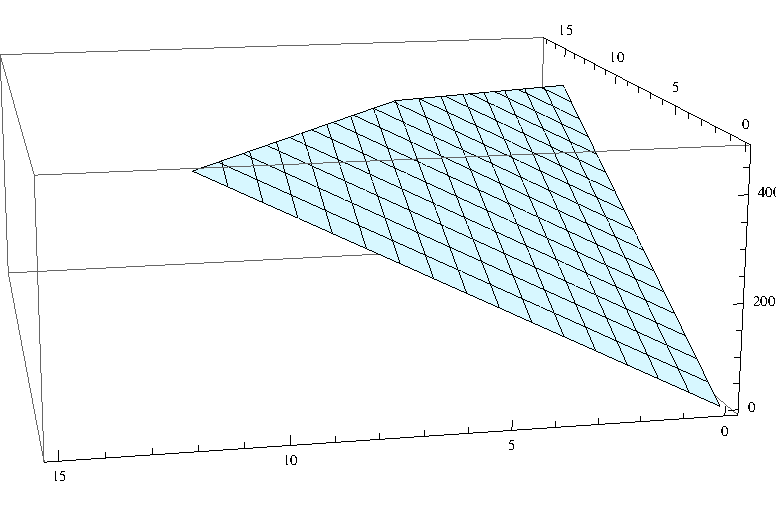
\includegraphics{functiononset}

\subsection{Problem LP.2}
\subsubsection{Question}
Show that the feasible set to the following problem permits the objective function to assume arbitrarily large values:
\[\begin{array}{ll}
\mathrm{Maximize}& 2x+y\\
\mathrm{Subject\ to:}& x-y \leq 3\\
& -3x +y \leq 1\\
& 0 \leq x, 0 \leq y.
\end{array}
\]

\subsubsection{Answer}
I claim in particular that each point of the  function $g(x)=y=2 x -1$ is contained within the feasible set given $x\geq 1/2$ and that the objective function tends to infinity along this funciton. 

\begin{proof}
Our the constraints on our feasible region may be rewritten as
\[ x-y \leq 3  \Leftrightarrow y \geq x - 3  \quad  -3x +y \leq 1 \Leftrightarrow y \leq 1 + 3x \]
Now just compute
\[ (2x -1)-(x-3) = x + 2   \]
which is greater than or equal to zero subject to $x\geq 1/2$ as claimed. Similarly we compute
\[ (1+3x ) - (2x - 1) = x +2\]
which is again greater than zero given $x \geq 1/2.$ It remains only to verify that our function has $x \geq 0$ and $y \geq 0$ for $x \geq 1/2$. That it satisfies this property for $x$ is implied directly from our restricting $x \geq 1/2$. Moreover since at $x = 1/2$ we get $y= 0$ and the $y$ value is strictly increasing in $x$ it is true as well that $y\geq 0$.

Now we just verify that our objective function tends to infinity along the function as claimed. Since as just demonstrated the portion of our function which has $x \geq 1/2$ is within the feasible set this will suffice to demonstrate that the objective function is not bounded in the feasible set.

For a given value of $x$ we may evaluate the objective function on $g(x)$ by 
 \[2x+y = 2x + 2x-1 = 4x -1 \] 
 and clearly we have 
\[\lim_{x \to  \infty} 4x -1 = \infty \]
so the objective function may assume arbitrarily large values on the feasible set as claimed.
\end{proof}

\end{document}
